\chapter{Literature Review: Neural Feature Matching}
\section{Review of Recent Methods}
In the last decade, neural networks have profoundly reshaped the landscape of
feature matching in all vision tasks, progressively replacing or complementing
traditional methods such as SIFT and ORB. Driven by the relentless pursuit of
computational efficiency, accuracy and adaptability, researches have turned to
deep learning as the logical solution to this challenge, leveraging its
powerful representation-learning capabilities to address longstanding issues in
classicals methods. particularly in fields demanding fast accurate processing,
such as robotics and augmented reality.

\section{ALIKE: Accurate and Lightweight Keypoint Detection and Descriptor Extraction}
To address the issue that existing keypoint detectors are non-differentiable
and cannot be optimized via back-propagation, this paper presents a novel,
partially differentiable keypoint detection module that outputs accurate
sub-pixel keypoints. The method uses a reprojection loss to directly optimize
these keypoints and a dispersity peak loss for regularization, ensuring
accuracy. Descriptors are also extracted at a sub-pixel level, trained with a
stable neural reprojection error loss. This entire process is handled by a
lightweight network capable of running at 95 frames per second on 640x480
images. The proposed method achieves performance equivalent to state-of-the-art
approaches in homography estimation, camera pose estimation, and visual
localization, while significantly reducing inference time.
\begin{figure}[h]
    \centering
    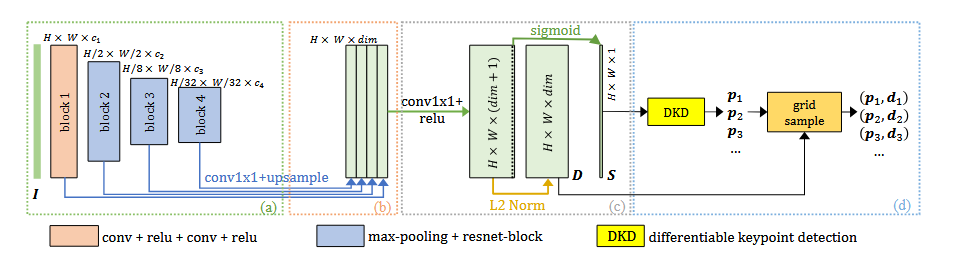
\includegraphics[width=\textwidth]{ressources/alike.png}
    \caption{architecture overview of ALIKE}
    \label{fig:alike}
\end{figure}
\subsection{Shared Feature Encoder}
At its base, ALIKE uses a lightweight Convolutional Neural Network (CNN) as its
backbone. This encoder takes an input image and processes it through several
convolutional layers to produce a set of shared feature maps. This design is
efficient because the computationally intensive process of feature extraction
is done only once, and the results are used for both the detection and
description tasks that follow. The focus is on creating a compact yet powerful
network that can run quickly on standard hardware.
\subsection{Keypoint Detection Head}
This is where ALIKE's main innovation lies. Instead of just identifying pixels
on a grid, the detection head is designed to find keypoints with sub-pixel
accuracy.
\begin{itemize}
    \item \textbf{Score Map Generation:} The detection head first produces a reliability or score map, where high values indicate a higher probability of a keypoint being present.
    \item \textbf{Partially Differentiable Detection:} To achieve sub-pixel accuracy, ALIKE performs a soft-argmax operation on local 2x2 patches of the score map. This process is "partially differentiable," meaning it allows the network to learn the precise location of a keypoint within a pixel's boundaries through back-propagation during training.
    \item \textbf{Loss Functions:} The detection process is optimized using two specific loss functions mentioned in the research:
          \begin{itemize}
              \item \textbf{Reprojection Loss:} This loss directly optimizes the sub-pixel coordinates of the keypoints, pushing them to be more geometrically consistent between different views of the same scene.
                    \begin{equation*}
                        \mathcal{L}_{\text{rep}} = \frac{1}{N} \sum_{i=1}^{N} \left\| p_i - \hat{p}_i \right\|_2
                    \end{equation*}
                    {\footnotesize
                    \begin{description}
                        \item[$\mathcal{L}_{\text{rep}}$] The Reprojection Loss value.
                        \item[$N$] The total number of matching keypoint pairs.
                        \item[$p_i$] The coordinates of a keypoint in the first image.
                        \item[$\hat{p}_i$] The coordinates of the corresponding keypoint from the second image, projected onto the first.
                        \item[$\left\| \cdot \right\|_2$] The L2 norm, which calculates the Euclidean distance between the two points.
                    \end{description}}
              \item \textbf{Dispersity Peak Loss:} This acts as a regularizer, encouraging the score map to have sharp, distinct peaks. This prevents keypoints from clumping together and ensures they are well-defined.
                    \begin{equation*}
                        \mathcal{L}_{\text{peak}} = \frac{1}{W \times H} \sum_{x,y} \left( \max(0, S(x,y) - \max_{\substack{dx,dy \in \{-1,0,1\}^2 \\ (dx,dy) \neq (0,0)}} S(x+dx, y+dy)) \right)
                    \end{equation*}
                    {\footnotesize
                    \begin{description}
                        \item[$\mathcal{L}_{\text{peak}}$] The Dispersity Peak Loss value.
                        \item[$W, H$] The width and height of the score map.
                        \item[$S(x,y)$] The score of the pixel at coordinate $(x,y)$.
                        \item[$\max_{\dots}$] The maximum score found within the 8-pixel neighborhood around the pixel $(x,y)$.
                        \item[$\max(0, \cdot)$] A rectifier (ReLU) ensuring the loss is non-negative. It penalizes pixels that are not a strict local maximum.
                    \end{description}}
          \end{itemize}
\end{itemize}
\subsection{Descriptor Extraction Head}
The descriptor head uses the shared feature maps from the encoder to generate a
distinctive descriptor for each detected keypoint.
\begin{itemize}
    \item \textbf{Sub-Pixel Descriptor Extraction:} To match the precision of the detection head, descriptors are also extracted in a sub-pixel manner. The network uses the precise sub-pixel coordinates generated by the detection head to sample from the descriptor feature map using bilinear interpolation. This ensures that the descriptor accurately represents the feature at its exact location, rather than just the nearest pixel center.
    \item \textbf{Training loss:} The descriptors are trained using a stable neural reprojection error loss. This loss function helps in learning descriptors that are robust to viewpoint and illumination changes, leading to more reliable matching.
\end{itemize}
By combining an efficient backbone with a novel, differentiable method for sub-pixel keypoint detection and description, ALIKE achieves state-of-the-art performance on various matching tasks while maintaining a very high processing speed (e.g., 95 FPS on 640x480 images).
\section{LightGlue: Local Feature Matching at Light Speed}
LightGlue is a deep neural network designed to efficiently and accurately match
local features between images. It builds upon the SuperGlue architecture by
introducing simpler, more efficient design choices that make it faster, more
memory-efficient, easier to train, and adaptive to the complexity of the image
pair. This adaptability allows LightGlue to process easier image pairs more
quickly, making it ideal for time-sensitive tasks like 3D reconstruction. The
model and its training code are publicly available.
\begin{figure}[h]
    \centering
    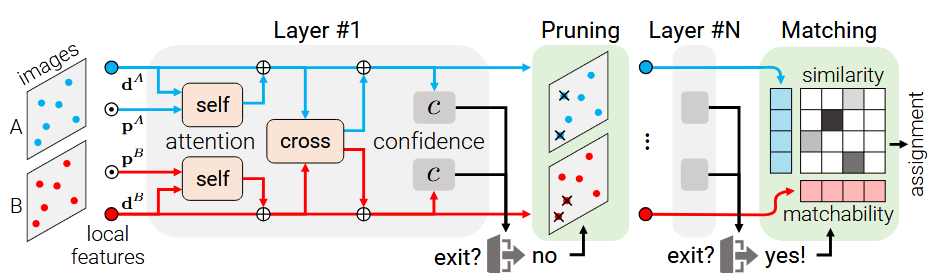
\includegraphics[width=\textwidth]{ressources/lightglue.png}
    \caption{architecture overview of LightGlue}
    \label{fig:lightglue}
\end{figure}
The architecture of LightGlue is designed to match sparse local features between two images efficiently while maintaining high accuracy. It builds upon the SuperGlue framework but introduces several key improvements that make it faster, easier to train, and more adaptive. Here's a breakdown of its core architectural components:
\subsection{Input Representation:}
LightGlue takes as input two sets of local features from both reference and
target image, each feature consists of normalized 2D coordinates and a
256-dimensional descriptor.
\subsection{Transformer-based Backbone: }
LightGlue uses a stack of Transformer layers to jointly process the features
from both images. Each layer includes:
\begin{itemize}
    \item \textbf{Self-Attention Mechanism:} This allows the model to capture long-range dependencies and relationships between features within each image.
    \item \textbf{Cross-Attention Mechanism:} This enables the model to learn correspondences between features from the reference and target images, enhancing the matching process.
\end{itemize}
\subsection{Lightweight Matching Head:}
After each layer, the network can predict similarity scores for all feature
pairs, as well as predict the matchability scores for each point (i.e., whether
a point is likely to have a corresponding point in the other image). It
combines similarity and matchability into a soft partial assignment matrix.
\subsection{Adaptive Inference:}
This is a unique feature of LightGlue, the ability to dynamically adjust the
computations by using:
\begin{itemize}
    \item \textbf{Adaptive Depth: }after each layer, a classifier predicts if a sufficient number of features
    \item \textbf{Adaptive Prunning:} the points predicted as confidently unmatchable are pruned from further processing, reducing computational load.
\end{itemize}
\section{XFeat: Accelerated Features for Lightweight Image Matching}
This work presents a new lightweight CNN structure that redefines the trade-off
between efficiency and accuracy for local feature extraction. In contrast to
existing deep models that need GPUs and/or hardware-specific tuning, XFeat
offers real-time performance on CPU-only systems by combining three components:
a featherweight backbone, a very light keypoint detection branch, and a match
refinement module that was new in its design. XFeat also uniquely has both
sparse and semi-dense matching modes, the first efficient model to do so, and
is suitable for visual localization and pose estimation. XFeat is typically
5–9× faster than other state-of-the-art methods, but offers similar or better
accuracy. The three design choices: growth of channel number tripled, early
resolution preservation, and coarse-to-fine refinement, contribute to high
quality matching for practical device constraints. It is a scalable,
lightweight and practical deep learning architecture for the real world.
\subsection{Featherweight Network Backbone}
The backbone of XFeat is designed to balance out computational efficiency and
representational accuracy:
\begin{itemize}
    \item \textbf{Channel Distribution Strategy}: The network begins with a minimal number of channels in the initial convolutional layers, where the spatial resolution is highest, to reduce computational load. As the spatial resolution decreases through subsequent layers, the number of channels is increased, following a tripling strategy (e.g starting with 4 channels and increasing up to 128 channels). This approach ensures that the network remains lightweight without compromising on feature extraction quality.
    \item \textbf{Convolutional Blocks}: The architecture comprises six convolutional blocks, each consisting of basic layers that include 2D convolutions  with kernel sizes ranging from 1 to 3, followed by ReLU activations and Batch Normalization. Strides of 2 are used for downsampling, \textbf{progressively reducing the spatial dimensions while increasing the depth of feature maps}
\end{itemize}
\subsection{Local Feature extraction}
XFeat employs specialized heads for different aspects of feature extraction:
\begin{itemize}
    \item \textbf{Descriptors Head}: This component extracts a dense feature map by merging multi-scale features from the encoder using a feature pyramid strategy. Intermediate representations at different scales (1/8, 1/16, and 1/32 of the original resolution) are upsampled and combined to enhance the receptive field without significantly increasing computational demands. A fusion block integrates these representations into the final feature map and an additional convolutional block generates a reliability map that indicates the confidence of each local feature.
    \item \textbf{Keypoint Head}: To efficiently detect keypoints, XFeat introduces a dedicated parallel branch focused on low-level image structures. The input image is represented as a 2D grid of 8x8 pixel  cells, each reshaped into 64-dimensional features. This representation preserves spatial granularity within individual cells while allowing rapid 1x1 convolutions for keypoint regression. After four convolutional layers, a keypoint embedding is obtained, encoding the distribution of keypoints within each cell.
\end{itemize}
\subsection{Dense Matching and Match Refinement}
XFeat includes a lightweight module for dense feature matching:
\begin{itemize}
    \item Match Refinement Module: This module refines coarse matches to achieve
          pixel-level accuracy without requiring high-resolution feature maps. It employs
          a simple MLP (Multi-Layer Perceptron), that predicts offsets between matching
          features, enabling efficient semi-dense matching suitable for
          resource-constrained settings.
\end{itemize}
\subsubsection{What is Mutual Nearest Neighbor?}
MNN, is a popular matching strategy used in image correspondence tasks to
robustly establish matches between two sets of local feature descriptors. It
helps ensure that matches are reciprocal, which greatly reduces false matches
compared to simple nearest neighbor methods. \subsubsection*{Mutual Nearest
    Neighbors (MNN) Algorithm}
\begin{itemize}
    \item \textbf{Compute Nearest Neighbors}: Given two feature sets:
          \begin{itemize}
              \item Set $A = \{a_1, a_2, \ldots, a_n\}$
              \item Set $B = \{b_1, b_2, \ldots, b_m\}$
          \end{itemize}
          For each feature $a_i \in A$, find its nearest neighbor in $B$ using:
          \[
              \text{NN}(a_i, B) = \arg\min_{b_j \in B} \|a_i - b_j\|
          \]
          where $\| \cdot \|$ is the Euclidean distance metric.
    \item \textbf{Reciprocal Check}
          For each candidate pair $(a_i, b_j)$ from Step 1:
          \begin{enumerate}
              \item Verify mutual nearest neighbor relationship:
                    \begin{align*}
                        \text{NN}(a_i, B) & = b_j \quad \text{(Original condition from Step 1)} \\
                        \text{NN}(b_j, A) & = a_i \quad \text{(Reciprocal condition)}
                    \end{align*}
              \item The pair $(a_i, b_j)$ is considered valid MNN iff both conditions hold [2][5]
          \end{enumerate}
    \item \textbf{Formal Definition}
          A pair $(a_i, b_j)$ is mutual nearest neighbors if:
          \[
              \forall b_k \in B, \|a_i - b_j\| \leq \|a_i - b_k\| \quad \land \quad \forall a_l \in A, \|b_j - a_i\| \leq \|b_j - a_l\|
          \]
          This bidirectional verification ensures correspondence stability in feature
          matching applications.
    \item \textbf{Discard Non-mutual Matches}
          If a pair does not fulfill mutual nearest neighbor criteria, it is discarded.
          After discarding non-mutual pairs, the final matched pairs are most robust against ambiguous matches.
\end{itemize}
\subsection{Sparse \& Semi-dense Matching}
The paper introduces two different matching modes based on previously explained
MNN, \textit{XFeat} and \textit{XFeat*}, they differ in the way they carry
image matching: \\

{\footnotesize
\begin{tabular}{|l|l|l|}
    \hline
    Aspect                & XFeat                                        & XFeat* (Star)                                \\
    \hline
    Matching strategy     & Sparse matching (keypoint-based)             & Semi-dense matching (coarse feature maps)    \\
    \hline
    Keypoints used        & Small set (up to 4,096 typically)            & Larger set (~10,000 typically)               \\
    \hline
    Refinement step       & No refinement                                & Match refinement (coarse-to-fine)            \\
    \hline
    Accuracy              & Good                                         & Higher (due to dense matching \& refinement) \\
    \hline
    Computational Cost    & Lower (faster, simpler)                      & Slightly higher (but still lightweight)      \\
    \hline
    Application scenarios & Visual localization, fast real-time matching & Pose estimation, dense scene                 \\
    \hline
\end{tabular}
}
\begin{enumerate}
    \item Sparse (XFeat) vs. Semi-dense Matching (XFeat*):
          \begin{itemize}
              \item \textit{XFeat} extracts a small set of keypoints (defaulting to 4096), uses Mutual Nearest Neighbor to match sparse features. It is fast and suitable for applications that prioritize speed and simplicity, such as visual localization or robotics.
              \item \textit{XFeat*} extracts semi-dense features, typically around 10,000 descriptors, and retains descriptors densely at different scales. It also performs matching in a coarse-to-fine manner, capturing more detailed correspondences across the image.
          \end{itemize}
    \item Match Refinement in \textit{XFeat*}: \\ XFeat* introduces a lightweight match
          refinement module: \\ Matches descriptors at a coarse level first. Then
          predicts pixel-level offsets to refine matches to exact pixel coordinates. This
          refinement significantly improves accuracy, especially in scenarios demanding
          precise correspondences (e.g., detailed scene reconstruction). \textit{XFeat}
          on the other hand has no such refinement; matches are at the original, coarse
          level.
    \item To resume: \\ {\footnotesize
          \begin{tabular}{|l|l|l|}
              \hline
              Metric             & XFeat (Basic) & XFeat* (Star)                            \\
              \hline
              Speed              & Very Fast     & Fast (slightly slower due to refinement) \\
              \hline
              Accuracy           & Good          & Higher accuracy                          \\
              \hline
              Density of matches & Sparse        & Semi-dense                               \\
              \hline
              Robustness         & Robust        & More robust                              \\
              \hline
          \end{tabular}
          }
          \begin{itemize}
              \item \textit{XFeat} is a fast, sparse matching approach focusing on extreme computational efficiency.
              \item \textit{XFeat*} is a semi-dense, refined matching approach, offering better accuracy at the slight expense of computational resources.
          \end{itemize}
\end{enumerate}
\section{Gaps and Limitations}
While there have been substantial advancements in neural-supported feature matching, frameworks such as ALIKE, XFeat, and LightGlue each encounter trade-offs limiting their suitability for purpose-built 2D image contexts. ALIKE does a great job at efficient keypoint detection and binary descriptors which makes it suitable for mobile and embedded contexts, but it is limited as it provides no built-in matching pipeline, and poor detection performance when the stimulus contains low-texture or synthetic scenarios, such as gaming or icon-based imagery. LightGlue employs an attention-based transformer model that makes it robust to perspective and lighting changes, but this comes at a high computational cost that also limits its adaptability to low-cost or low-latency environments for rapid feature matching. This state of play lays bare a glaring gap in the research alignment: there is no single feature matching framework that combines the benefit of speed (e.g., ALIKE and XFeat) with the ability to adaptively and robustly handle image distortion to the extent of (or more) than LightGlue, and is specifically optimized for "2D" applications, such as icon localization, synthetic-to-real matching, and dynamic in-game overlays—where conventional 3D priors and richly textured cues are often absent or unreliable. XFeat improves upon some of its limitations by adopting a more integrated process to detection, description, and matching in a lightweight end-to-end model that demonstrates impressive efficiency gains when doing computationally expensive matching comparisons, however, its performance is limited when considering view and lighting changes or changing imagery states when the model is representative of highly structured and realistic 2D datasets.